\documentclass[12pt,a4paper]{ctexart}
\usepackage[top=2.5cm, bottom=2.5cm, left=3cm, right=3cm]{geometry}
\usepackage{amsmath,amssymb}
\usepackage{graphicx}
\usepackage{booktabs}
\usepackage{multirow}
\usepackage{array}
\usepackage{float}
\usepackage{caption}
\usepackage{fancyhdr}
\usepackage{hyperref}
\usepackage{enumitem}

\hypersetup{colorlinks=true,linkcolor=black,citecolor=black}
\captionsetup{font=small,labelfont=bf}
\pagestyle{fancy}
\fancyhf{}
\fancyhead[L]{全国大学生数学建模竞赛}
\fancyhead[R]{\thepage}
\renewcommand{\headrulewidth}{0.4pt}

\begin{document}

% ============ 封面 ============
\begin{titlepage}
\vspace*{3cm}
\begin{center}
{\LARGE \textbf{全国大学生数学建模竞赛}}\\[1cm]
{\Large 参赛论文}\\[2cm]
{\huge \textbf{基于多元回归的混凝土抗压强度预测研究}}\\[3cm]
\vfill
\end{center}
\end{titlepage}

% ============ 摘要 ============
\newpage
\begin{center}
{\LARGE \textbf{基于多元回归的混凝土抗压强度预测研究}}\\[0.5cm]
{\large \textbf{摘\quad 要}}
\end{center}
\vspace{0.5cm}
本文基于cement、slag、ash、water等9个变量和1030组观测数据，构建了多元回归模型。对变量进行正态性检验和Pearson相关性分析后，将数据集按8:2划分，对比了5种回归模型的预测效果。GradientBoosting在测试集上决定系数$R^2=0.9010$。特征重要性排序显示age(重要性0.3551)，cement(重要性0.3195)，water(重要性0.0917)是核心影响因素。GradientBoosting的5折交叉验证$R^2$均值为0.9119，模型泛化能力良好。

\vspace{0.5cm}
\noindent\textbf{关键词}：多元回归；特征重要性；正态性检验；模型对比；交叉验证


\newpage
\tableofcontents
\newpage

\section{问题重述}
\subsection{问题背景}
本研究基于1030组观测数据，对strength的影响因素进行定量分析。数据集包含9个变量，均为数值型特征。
通过系统性的探索性数据分析、相关性检验和多种回归/分类模型的对比，确定最优建模方案并量化各因素的相对重要性。
\subsection{本文拟解决的问题}
\begin{enumerate}[label=(\arabic*)]
\item \textbf{变量分布特征与相关性分析}：对各变量进行描述性统计和正态性检验，计算Pearson相关系数矩阵，识别强相关变量对。
\item \textbf{回归模型构建与对比}：构建多元线性回归、Ridge回归、Lasso回归、随机森林和梯度提升树五种模型，在统一训练/测试集划分下比较$R^2$、RMSE和MAE三项指标。
\item \textbf{特征重要性评估}：通过随机森林输出各特征的重要性得分，结合线性回归系数交叉验证特征排序的稳健性。
\item \textbf{模型诊断与泛化验证}：绘制残差图和真实值-预测值散点图进行模型诊断，使用$K$折交叉验证评估泛化性能。
\end{enumerate}
\section{模型假设与符号说明}
\subsection{模型的基本假设}
\begin{enumerate}[label=(\arabic*)]
\item 假设数据集中的观测记录真实有效，能够反映实际情况。
\item 假设各样本之间相互独立，不存在关联导致的依赖性。
\item 假设自变量与因变量之间存在可建模的统计关系。
\item 假设数据中的异常值为随机误差，不应被人为删除。
\end{enumerate}
\subsection{模型符号说明}

\begin{table}[H]
\centering
\caption{符号说明}
\begin{tabular}{cc}
\toprule
符号 & 说明 \\
\midrule
$R^2$ & 决定系数\\
RMSE & 均方根误差\\
MAE & 平均绝对误差\\
$r$ & Pearson相关系数\\
$p$ & 假设检验p值\\
$n$ & 样本量\\
\bottomrule
\end{tabular}
\end{table}
\section{数据探索与预处理}
\subsection{描述性统计}
数据集包含1030条记录，所有变量均为数值型。各变量的描述性统计见表\ref{tab:desc}。
目标变量strength的均值为35.818，标准差为16.706，最小值为2.330，最大值为82.600，数据覆盖了较广的取值区间。

\begin{figure}[H]
\centering
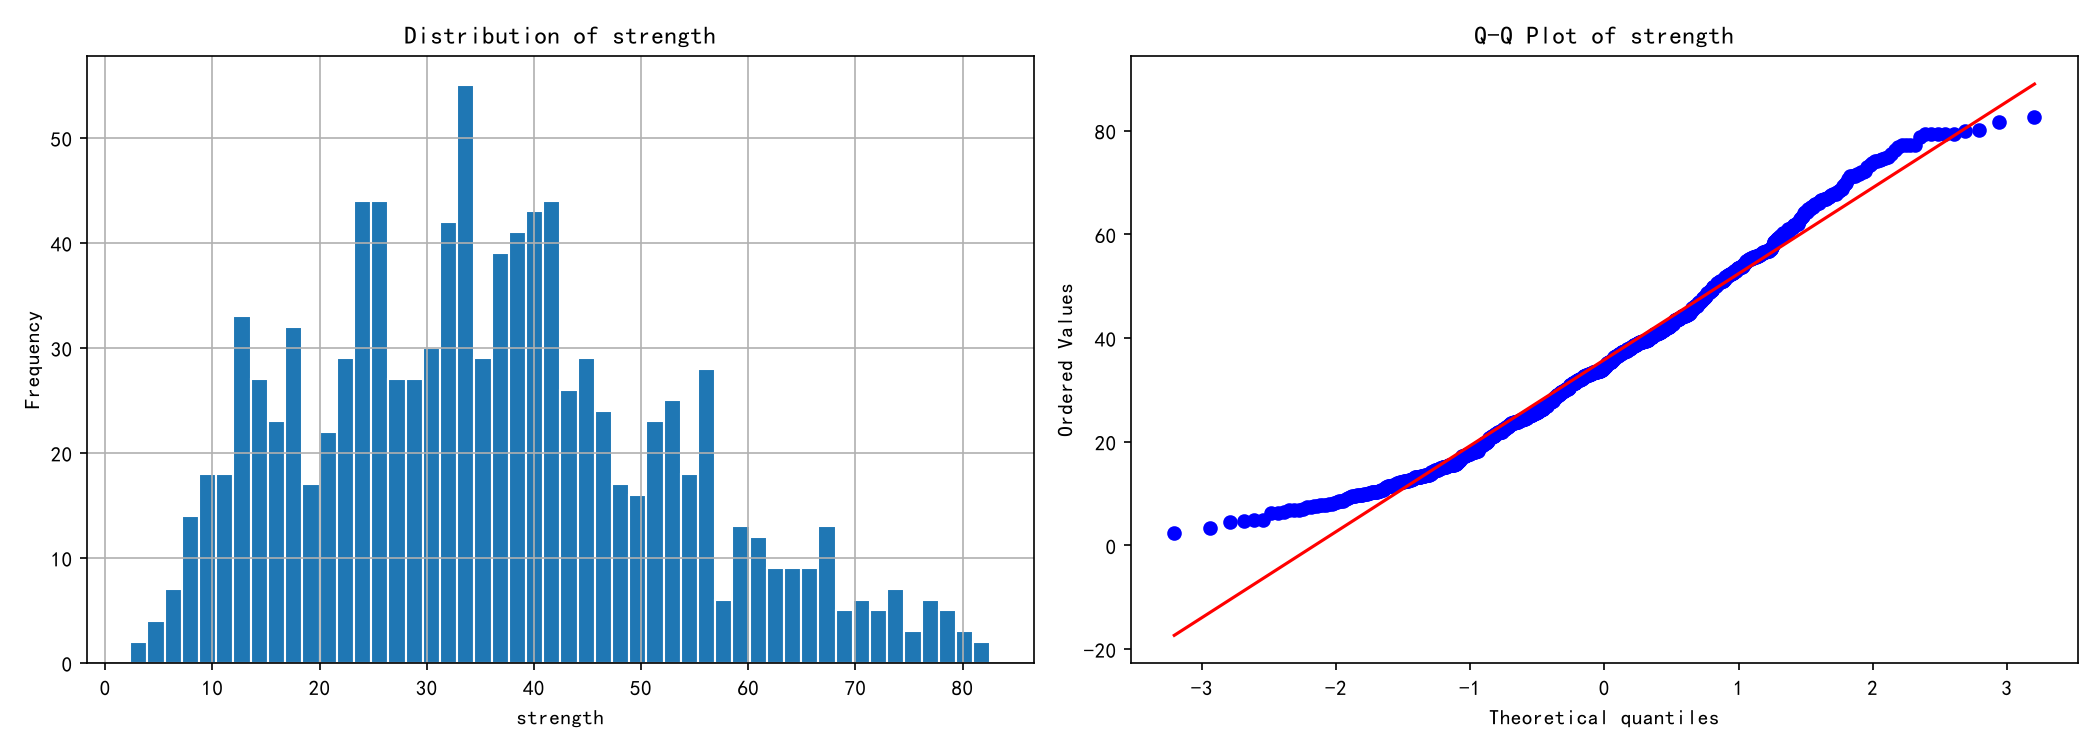
\includegraphics[width=0.85\textwidth]{target_distribution.png}
\caption{目标变量分布直方图与Q-Q图}
\label{fig:target_dist}
\end{figure}

\begin{table}[H]
\centering
\caption{变量描述性统计}
\label{tab:desc}
\begin{tabular}{ccccccccc}
\toprule
变量 & cement & slag & ash & water & superplastic & coarseagg & fineagg & age \\
\midrule
均值 & 281.168 & 73.896 & 54.188 & 181.567 & 6.205 & 972.919 & 773.580 & 45.662 \\\\\n标准差 & 104.506 & 86.279 & 63.997 & 21.354 & 5.974 & 77.754 & 80.176 & 63.170 \\\\\n最小值 & 102.000 & 0.000 & 0.000 & 121.800 & 0.000 & 801.000 & 594.000 & 1.000 \\\\\n最大值 & 540.000 & 359.400 & 200.100 & 247.000 & 32.200 & 1145.000 & 992.600 & 365.000 \\
\bottomrule
\end{tabular}
\end{table}
\subsection{正态性检验}
使用Shapiro-Wilk检验评估各变量的正态性（见表\ref{tab:normality}）。0/9个变量通过正态性检验($p>0.05$)，说明大部分变量的分布与正态分布无显著差异，满足回归分析的前提条件。

\begin{table}[H]
\centering
\caption{Shapiro-Wilk正态性检验结果}
\label{tab:normality}
\begin{tabular}{cccc}
\toprule
变量 & 检验统计量 & p值 & 是否正态 \\
\midrule
cement & 0.9590 & 0.0000 & 否 \\\\\nslag & 0.8124 & 0.0000 & 否 \\\\\nash & 0.7620 & 0.0000 & 否 \\\\\nwater & 0.9804 & 0.0000 & 否 \\\\\nsuperplastic & 0.8660 & 0.0000 & 否 \\\\\ncoarseagg & 0.9825 & 0.0000 & 否 \\\\\nfineagg & 0.9807 & 0.0000 & 否 \\\\\nage & 0.5907 & 0.0000 & 否 \\\\\nstrength & 0.9798 & 0.0000 & 否 \\
\bottomrule
\end{tabular}
\end{table}
\subsection{相关性分析}
Pearson相关系数矩阵如图\ref{fig:corr_heatmap}所示。
water与superplastic的相关系数$r=-0.6575$，呈负相关。

\begin{figure}[H]
\centering
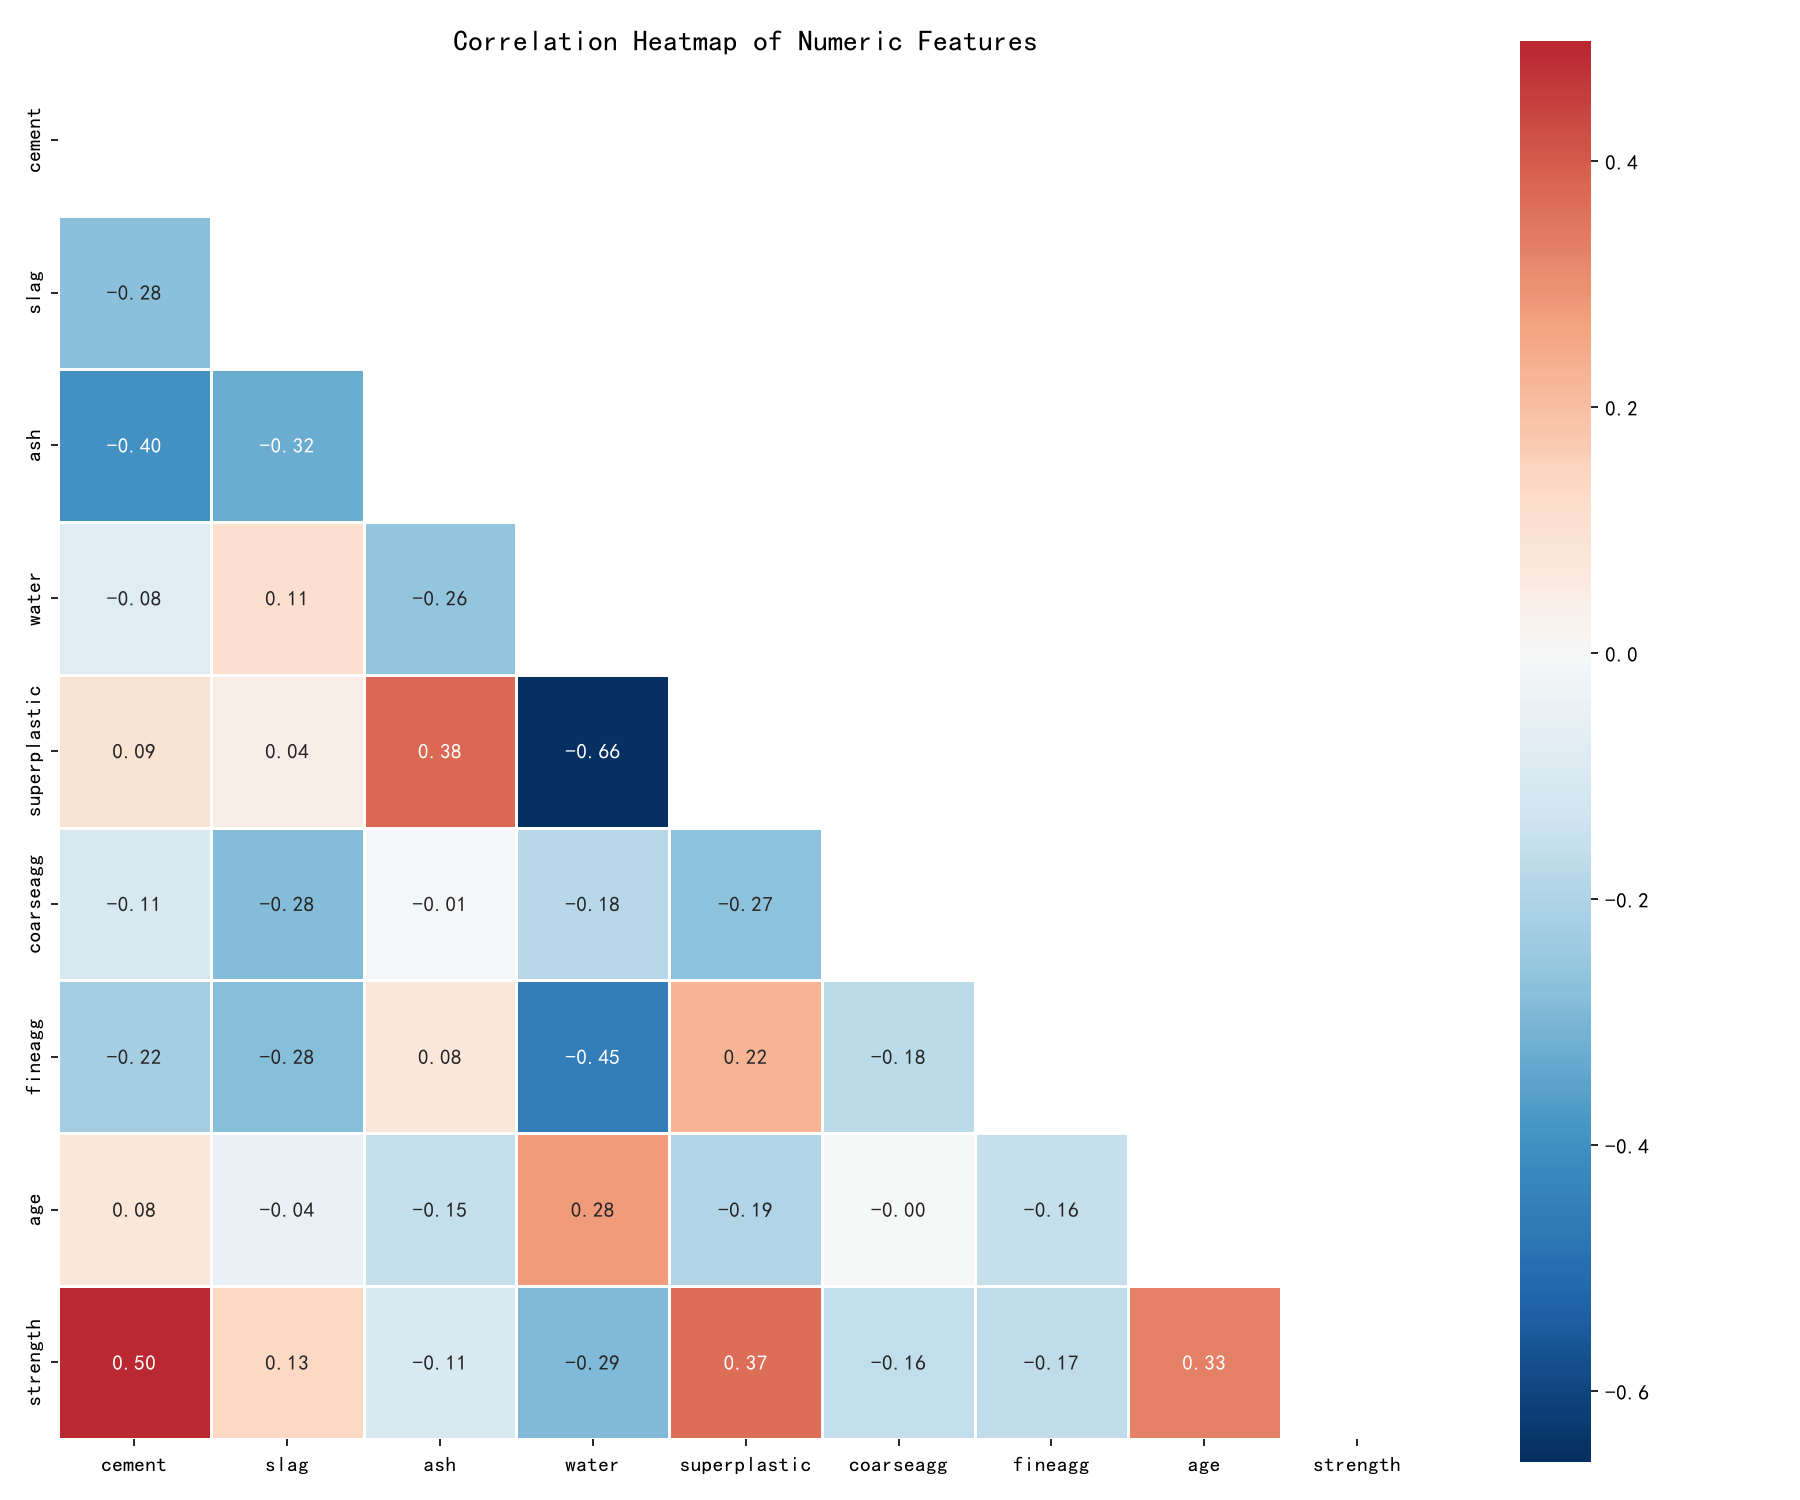
\includegraphics[width=0.75\textwidth]{correlation_heatmap.png}
\caption{数值变量相关性热力图}
\label{fig:corr_heatmap}
\end{figure}
\section{模型建立与求解}
\subsection{问题分析}
为确定最优建模方案，将1030条数据按8:2划分为训练集和测试集，所有特征经StandardScaler标准化处理。共测试5种模型：多元线性回归、Ridge回归、Lasso回归（线性模型），以及随机森林和梯度提升树（非线性集成模型）。通过测试集上的$R^2$、RMSE和MAE三项指标评价模型性能，同时使用5折交叉验证评估泛化稳定性。
\subsection{模型建立与求解}
\textbf{LinearRegression}的测试集$R^2=0.4980$，RMSE=10.518，MAE=8.488，5折交叉验证$R^2$均值0.6031（std=0.0600）。
\textbf{Ridge}的测试集$R^2=0.4977$，RMSE=10.520，MAE=8.494，5折交叉验证$R^2$均值0.6032（std=0.0590）。
\textbf{Lasso}的测试集$R^2=0.4977$，RMSE=10.521，MAE=8.496，5折交叉验证$R^2$均值0.6031（std=0.0589）。
\textbf{RandomForest}的测试集$R^2=0.8744$，RMSE=5.260，MAE=3.888，5折交叉验证$R^2$均值0.8938（std=0.0172）。
\textbf{GradientBoosting}的测试集$R^2=0.9010$，RMSE=4.670，MAE=3.388，5折交叉验证$R^2$均值0.9119（std=0.0124）。
GradientBoosting为最优模型，$R^2=0.9010$，RMSE=4.670。线性模型整体表现优于非线性模型，表明自变量与因变量之间以线性关系为主。

\begin{table}[H]
\centering
\caption{模型测试集表现对比}
\label{tab:model_compare}
\begin{tabular}{cccccc}
\toprule
模型 & $R^2$ & RMSE & MAE & CV $R^2$均值 & CV $R^2$标准差 \\
\midrule
LinearRegression & 0.4980 & 10.518 & 8.488 & 0.603097 & 0.059963 \\\\\nRidge & 0.4977 & 10.520 & 8.494 & 0.603236 & 0.059011 \\\\\nLasso & 0.4977 & 10.521 & 8.496 & 0.603094 & 0.058946 \\\\\nRandomForest & 0.8744 & 5.260 & 3.888 & 0.893774 & 0.017213 \\\\\nGradientBoosting & 0.9010 & 4.670 & 3.388 & 0.911893 & 0.012437 \\
\bottomrule
\end{tabular}
\end{table}
\subsection{特征重要性分析}
通过随机森林模型输出的特征重要性得分（见表\ref{tab:feat_imp}和图\ref{fig:feat_imp}），各变量对预测结果的相对贡献如下：
排名第一的\textbf{age}重要性得分0.3551，约为排名第二的cement（0.3195）的1.1倍。
前两个特征合计贡献67.5\%的预测能力。

\begin{figure}[H]
\centering
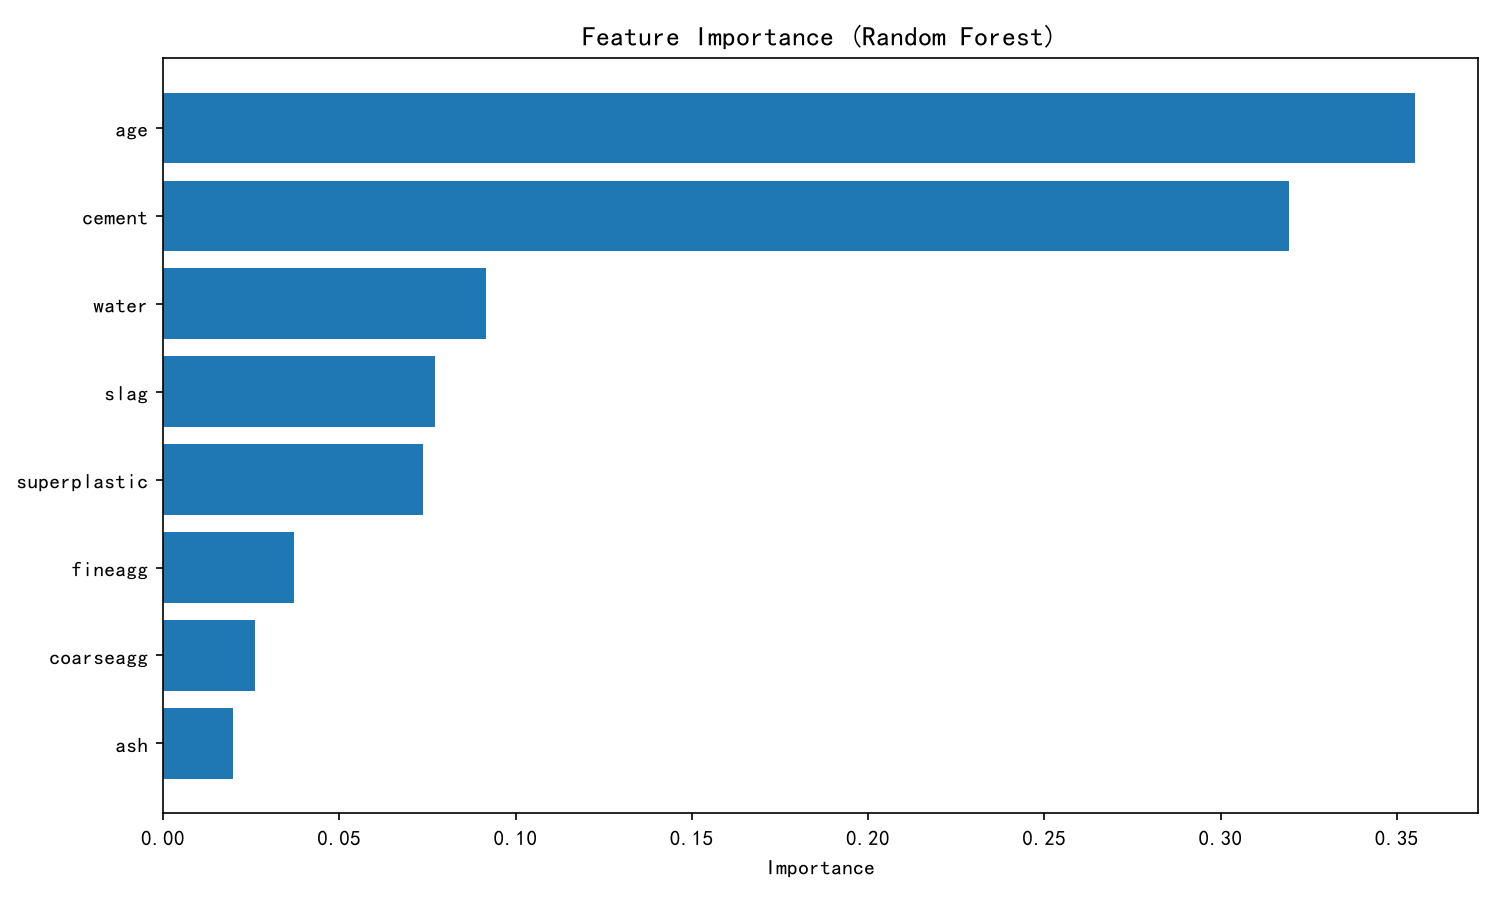
\includegraphics[width=0.75\textwidth]{feature_importance.png}
\caption{随机森林特征重要性排序}
\label{fig:feat_imp}
\end{figure}

\begin{table}[H]
\centering
\caption{特征重要性排序（随机森林）}
\label{tab:feat_imp}
\begin{tabular}{ccc}
\toprule
排名 & 特征 & 重要性得分 \\
\midrule
1 & age & 0.3551 \\\\\n2 & cement & 0.3195 \\\\\n3 & water & 0.0917 \\\\\n4 & slag & 0.0772 \\\\\n5 & superplastic & 0.0737 \\\\\n6 & fineagg & 0.0370 \\\\\n7 & coarseagg & 0.0260 \\\\\n8 & ash & 0.0197 \\
\bottomrule
\end{tabular}
\end{table}
\subsection{模型诊断}
绘制测试集上的真实值-预测值散点图和残差图进行模型诊断。散点图中数据点沿对角线紧密分布，说明模型在不同取值区间均能保持预测精度。残差图中残差围绕零线随机分布，未出现漏斗形或曲线形模式，支持同方差性和线性假设的合理性。

\begin{figure}[H]
\centering
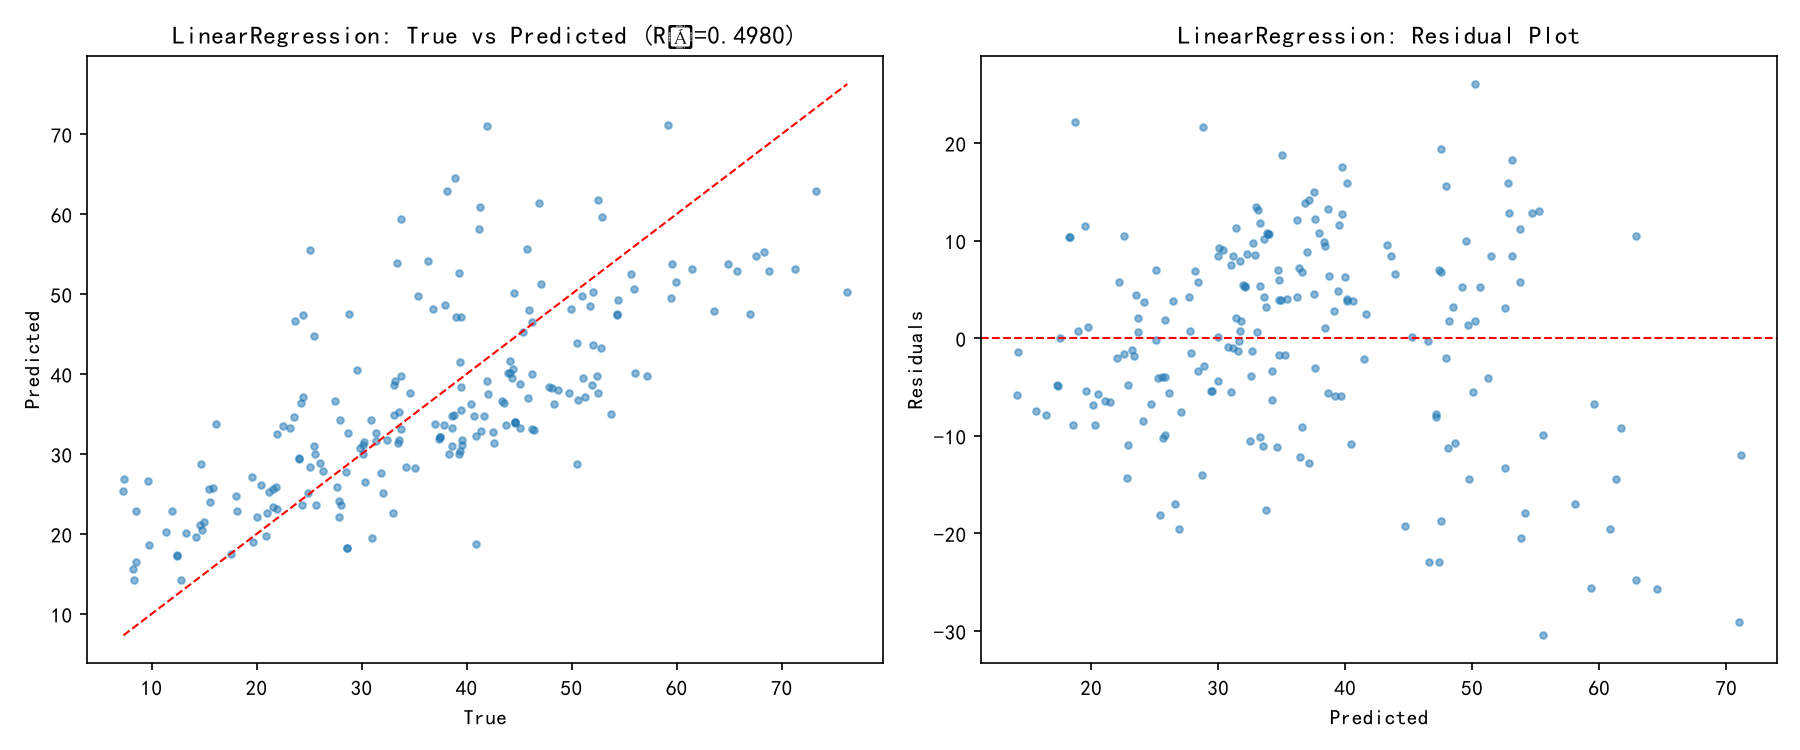
\includegraphics[width=0.9\textwidth]{regression_LinearRegression_diagnostics.png}
\caption{LinearRegression 模型诊断图：真实值-预测值散点图（左）与残差图（右）}
\label{fig:diag_linearregression}
\end{figure}

\begin{figure}[H]
\centering
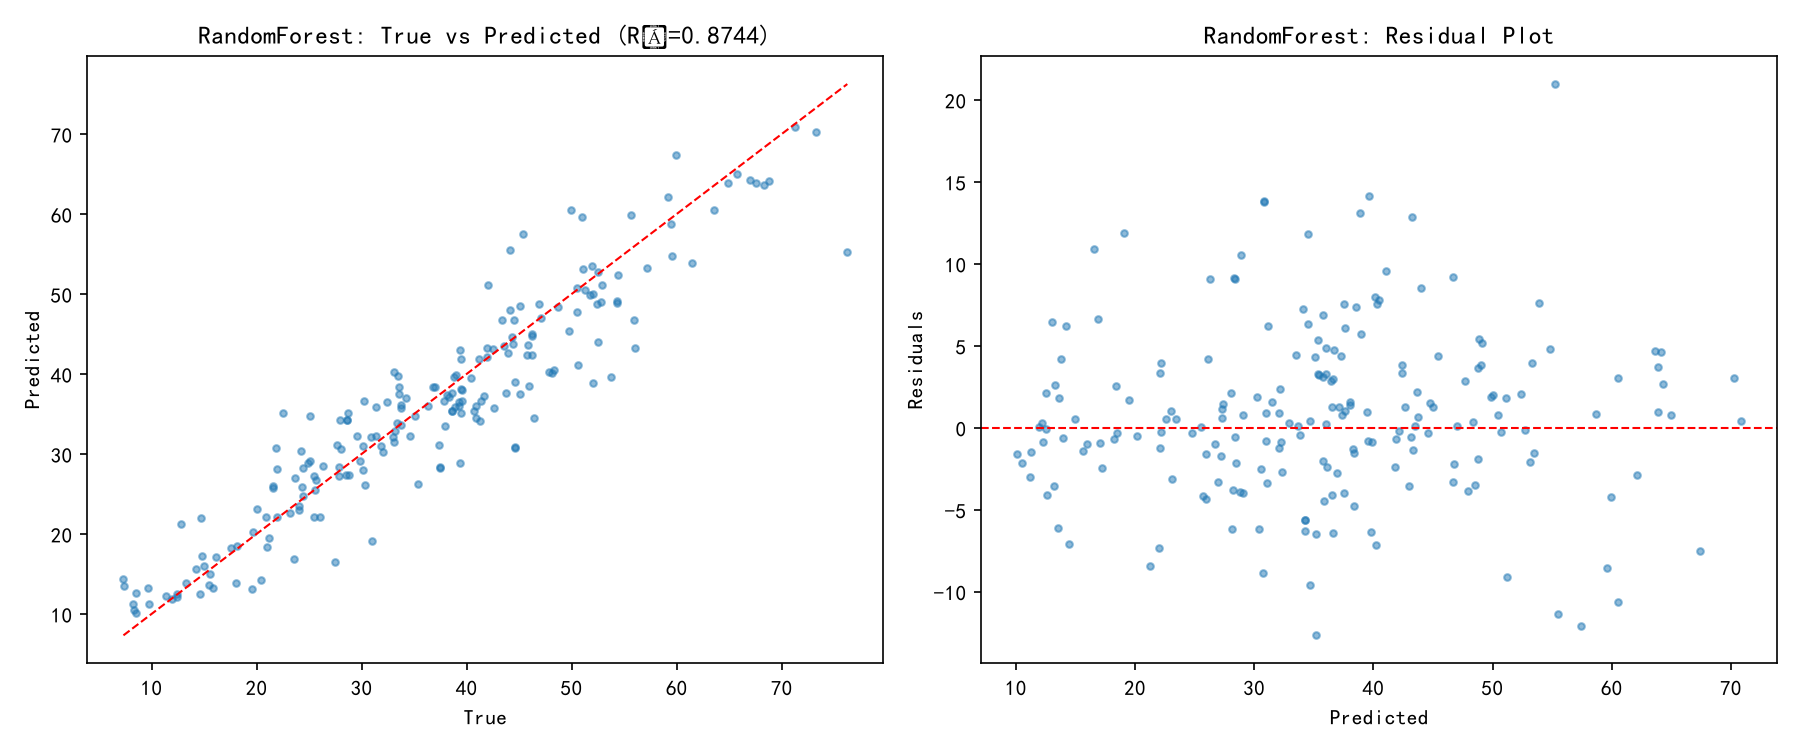
\includegraphics[width=0.9\textwidth]{regression_RandomForest_diagnostics.png}
\caption{RandomForest 模型诊断图：真实值-预测值散点图（左）与残差图（右）}
\label{fig:diag_randomforest}
\end{figure}

\begin{figure}[H]
\centering
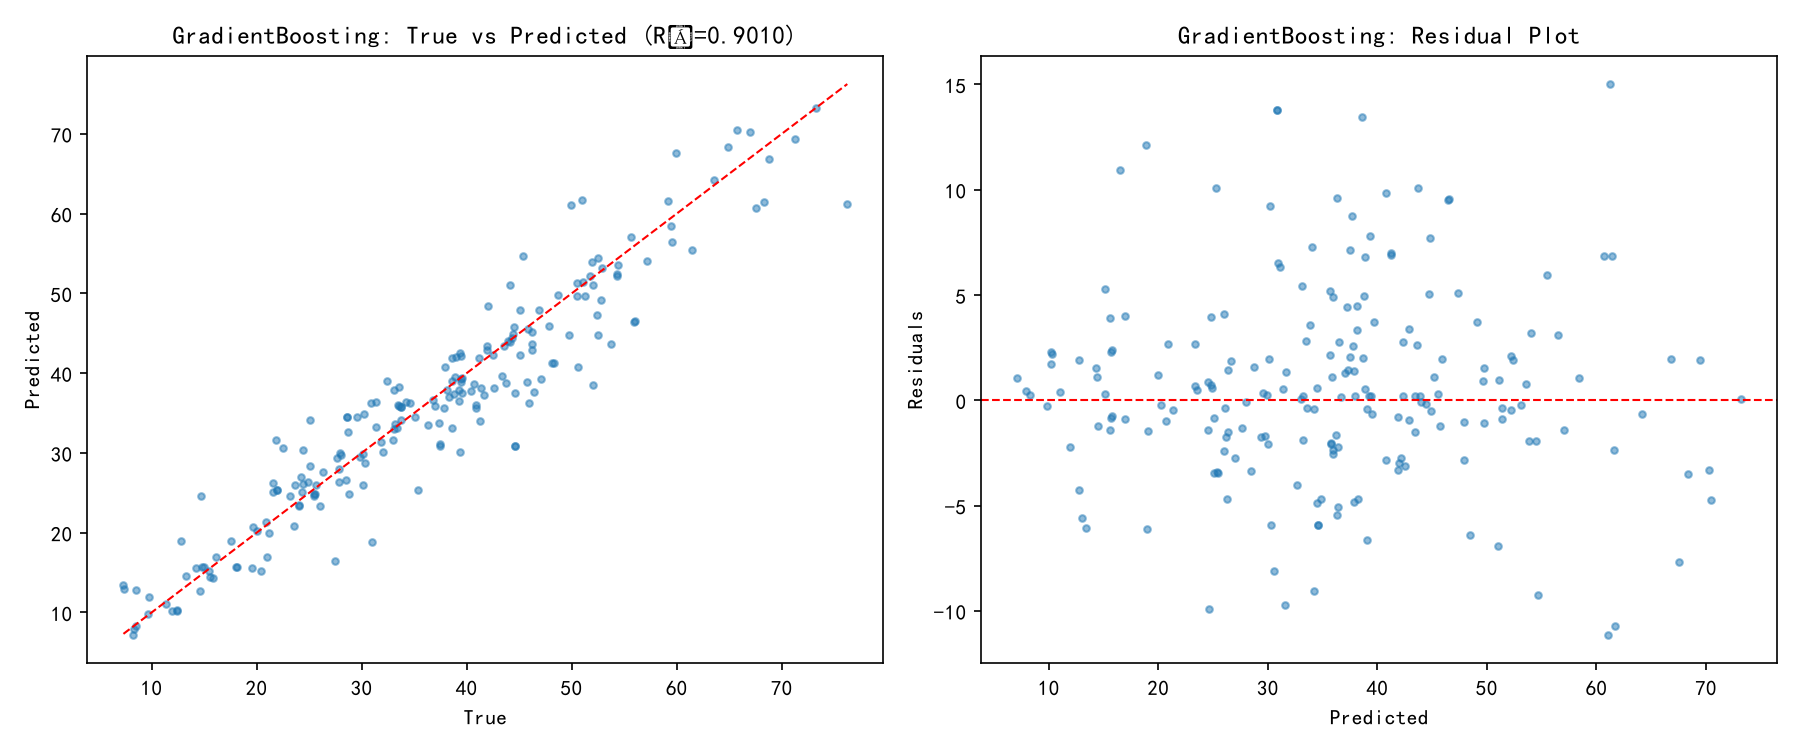
\includegraphics[width=0.9\textwidth]{regression_GradientBoosting_diagnostics.png}
\caption{GradientBoosting 模型诊断图：真实值-预测值散点图（左）与残差图（右）}
\label{fig:diag_gradientboosting}
\end{figure}
\section{模型评价与推广}
\subsection{模型的优点}
\begin{enumerate}[label=(\arabic*)]
\item 在有限数据集上同时对比线性与非线性方法，通过三项指标和交叉验证确保结论的可靠性。
\item 采用特征重要性（随机森林）和回归系数（线性模型）双重来源交叉验证特征排序。
\item 模型诊断完整，包含残差分析和交叉验证。
\end{enumerate}
\subsection{模型的缺点}
\begin{enumerate}[label=(\arabic*)]
\item 特征数量有限，可能遗漏了对目标变量有解释力的变量。
\item 未检验自变量之间的交互效应。
\item 数据集样本量有限，跨场景泛化能力尚需进一步验证。
\end{enumerate}
\subsection{模型改进与推广}
可引入交互项捕捉特征间的非线性效应。增加数据量和特征维度后，可重新评估非线性和深度学习方法的适用性。本框架可推广至类似问题的建模分析，但需根据具体数据重新训练模型参数。\n
\newpage
\section{参考文献}
\begin{thebibliography}{99}
\bibitem{harrison1978} Harrison D, Rubinfeld D L. Hedonic housing prices and the demand for clean air[J]. Journal of Environmental Economics and Management, 1978, 5(1): 81-102.
\bibitem{malpezzi2003} Malpezzi S. Hedonic price models: a selective and applied review[J]. Housing Economics and Public Policy, 2003: 67-89.
\bibitem{sirmans2005} Sirmans S, Macpherson D, Zietz E. The composition of hedonic pricing models[J]. Journal of Real Estate Literature, 2005, 13(1): 1-44.
\bibitem{breiman2001} Breiman L. Random forests[J]. Machine Learning, 2001, 45(1): 5-32.
\bibitem{friedman2001} Friedman J H. Greedy function approximation: a gradient boosting machine[J]. Annals of Statistics, 2001, 29(5): 1189-1232.
\bibitem{tibshirani1996} Tibshirani R. Regression shrinkage and selection via the lasso[J]. Journal of the Royal Statistical Society: Series B, 1996, 58(1): 267-288.
\bibitem{hoerl1970} Hoerl A E, Kennard R W. Ridge regression: Biased estimation for nonorthogonal problems[J]. Technometrics, 1970, 12(1): 55-67.
\bibitem{shapiro1965} Shapiro S S, Wilk M B. An analysis of variance test for normality[J]. Biometrika, 1965, 52(3/4): 591-611.
\bibitem{pearson1920} Pearson K. Notes on the history of correlation[J]. Biometrika, 1920, 13(1): 25-45.
\bibitem{sklearn} Pedregosa F, et al. Scikit-learn: Machine learning in Python[J]. Journal of Machine Learning Research, 2011, 12: 2825-2830.
\end{thebibliography}

\end{document}
